
%%Source: Pruebas_environment-infrastructure-test-subtype_score_hpc_uniq-paralell_sdo_uniq.csv

% 

%\begin{figure*}[ht!]
%%https://www.overleaf.com/learn/latex/Positioning_of_Figures
    \centerline{
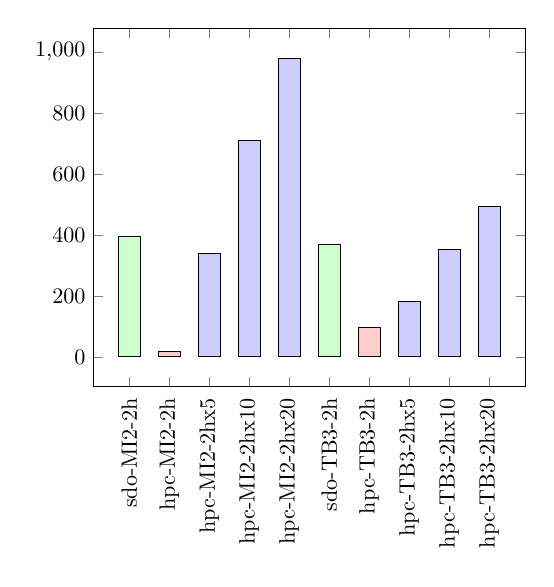
\begin{tikzpicture}[scale=0.80]
\begin{axis}[
    symbolic x coords={sdo-MI2-2h,hpc-MI2-2h, hpc-MI2-2hx5, hpc-MI2-2hx10, hpc-MI2-2hx20, sdo-TB3-2h, hpc-TB3-2h, hpc-TB3-2hx5, hpc-TB3-2hx10, hpc-TB3-2hx20},
    bar width=10pt,
    xtick=data,
    x tick label style={rotate=90, anchor=east , inner sep=5pt}]
    \addplot[ybar,fill=blue!20] coordinates {
        (sdo-MI2-2h,0)  %% Workaround: para tener leyenda en el eje x
        (hpc-MI2-2h,0)  %% Workaround: para tener leyenda en el eje x
        (hpc-MI2-2hx5,340)
        (hpc-MI2-2hx10,710)
        (hpc-MI2-2hx20,980)
        (sdo-TB3-2h,0)  %% Workaround: para tener ejex en el eje x
        (hpc-TB3-2h,0)  %% Workaround: para tener ejex en el eje x
        (hpc-TB3-2hx5,183)
        (hpc-TB3-2hx10,353)
        (hpc-TB3-2hx20,494)
    };
     %\addlegendentry{Paralell task}
    \addplot[ybar,fill=red!20] coordinates {
        (sdo-MI2-2h,0)  %% Workaround: para tener leyenda en el eje x
        (hpc-MI2-2h,16.666666671)
        (sdo-TB3-2h,0)  %% Workaround: para tener ejex en el eje x
        (hpc-TB3-2h,96.333333331)
    };
    \addplot[ybar,fill=green!20] coordinates {
        (sdo-MI2-2h,395)
        (sdo-TB3-2h,367.6666667)
    };
    
    %\addlegendentry{Unique task}
    
\end{axis}
\end{tikzpicture}}
    % El contenido de legendbox se cambia en package.tex linea 55 donde se define el robustcommand usado para dibujarlo.
%    \caption{The diagram presents a comparison between: \legendbox{green} the average score of 2h single tasks using a standalone computer (sdo), \legendbox{red} the average score of 2h single tasks using the singularity environment in the HPC infrastructure, and \legendbox{blue} parallel tasks using the score accumulated by the n parallel jobs in the HPC.}
%    %\caption{Comparativa entre tareas paralelas  \legendbox{blue} usando el score acumulado por las n tareas paraleleas  y el socre medio de tareas unicas de 2h \legendbox{red}  usando el entorno singularity en la infraestructura de HPC. Y el score medio de 2h en tareas unicas \legendbox{green} usando sdo.}
%    \label{fig:Barplot_score_by_paralell-unique_hpc}
%\end{figure*}